\documentclass[conference]{IEEEtran}
\IEEEoverridecommandlockouts
% Paquetes para español
\usepackage[spanish]{babel}
\usepackage[utf8]{inputenc}
\usepackage{cite}
\usepackage{amsmath,amssymb,amsfonts}
\usepackage{algorithmic}
\usepackage{graphicx}
\usepackage{textcomp}
\usepackage{booktabs}
\usepackage{xcolor}
% Si falta una imagen, muestra un recuadro en lugar de detener la compilación
\let\oldincludegraphics\includegraphics
\renewcommand{\includegraphics}[2][]{\IfFileExists{#2}{\oldincludegraphics[#1]{#2}}{\fbox{\parbox{0.8\columnwidth}{\centering Imagen faltante:\\ \texttt{\detokenize{#2}}}}}}
\def\BibTeX{{\rm B\kern-.05em{\sc i\kern-.025em b}\kern-.08em
    T\kern-.1667em\lower.7ex\hbox{E}\kern-.125emX}}
\begin{document}

\title{ADALINE: Clasificación binaria del estado de peso a partir de altura y peso}

\author{\IEEEauthorblockN{1\textsuperscript{st} Oscar Alberto Gallo García}
\IEEEauthorblockA{\textit{M. C. en Robótica e Inteligencia Artificial} \\
\textit{Centro Universitario de Ciencias Exactas e Ingenierías}\\
Guadalajara, México \\
oscar.gallo5770@alumnos.udg.mx}
}

\maketitle

\begin{abstract}
    Se implementó desde cero una neurona ADALINE (\textit{Adaptive Linear Neuron})
    entrenada con la regla delta de Widrow--Hoff mediante descenso de gradiente
    estocástico (SGD). La red se utilizó para clasificar a adultos mexicanos en
    dos clases, \textit{bajo peso o peso normal} y \textit{sobrepeso u obesidad},
    usando únicamente su altura y su peso, medidos en la ENSANUT 2022. El índice de masa corporal (IMC)
    se empleó solo para construir las etiquetas. Se estudió el efecto de la razón de
    aprendizaje $\eta$ y del método de escalamiento sobre la convergencia, y se
    analizó la frontera lineal aprendida respecto a la frontera teórica
    $m=25h^2$. El modelo final alcanzó una exactitud de $88.39\%$ en el
    conjunto de prueba.
\end{abstract}

\begin{IEEEkeywords}
ADALINE, regla delta, LMS, descenso de gradiente estocástico, clasificación lineal, IMC
\end{IEEEkeywords}

\section{Introducción}
ADALINE fue propuesto por Widrow y Hoff como una unidad lineal adaptativa. A
diferencia del perceptrón, durante el entrenamiento utiliza directamente la
salida lineal de la neurona para calcular el error, lo que permite formular el
aprendizaje como la minimización de una función de costo cuadrática y derivar
la regla de actualización mediante descenso de gradiente
\cite{b1,b2,b3}. Esta idea es la base de los métodos de entrenamiento de
redes multicapa \cite{b4}.

En esta práctica se construye un problema de clasificación binaria con datos
reales. A partir de la altura $h$ y el peso $m$ de cada persona se busca
decidir si su IMC es menor o mayor-igual que $25$. Como la frontera ideal
$m=25h^2$ es una parábola, el problema no es estrictamente lineal en el plano
altura--peso; esto permite observar hasta dónde llega una sola unidad lineal y
dónde aparecen sus errores.

\section{Desarrollo}

\subsection{Modelo ADALINE}
La salida lineal de la neurona para el patrón $k$ es
\begin{align}
    \label{eq:salida}
    y(k) = \mathbf{W}^\top(k)\mathbf{X}(k) + b(k),\quad
    \mathbf{X}(k)=\begin{bmatrix}\text{altura}(k)\\ \text{peso}(k)\end{bmatrix}
\end{align}
con función de activación identidad. El error instantáneo es
$e(k)=d(k)-y(k)$ y la función de costo es el error cuadrático
\begin{align}
    \label{eq:costo}
    E(k)=\tfrac{1}{2}e^2(k)=\tfrac{1}{2}\left[d(k)-y(k)\right]^2.
\end{align}
Aplicando la regla de la cadena,
$\partial E/\partial w_i = -e(k)x_i(k)$ y $\partial E/\partial b=-e(k)$, por lo que
el descenso de gradiente produce la regla delta (Widrow--Hoff / LMS):
\begin{align}
    \label{eq:deltaW}
    \mathbf{W}(k+1) &= \mathbf{W}(k) + \eta\, e(k)\,\mathbf{X}(k)\\
    \label{eq:deltab}
    b(k+1) &= b(k) + \eta\, e(k)
\end{align}
La función signo se usa únicamente después del entrenamiento para convertir la
salida continua en una clase:
\begin{align}
    \label{eq:signo}
    \hat{d}(k)=\begin{cases}+1, & y(k)\geq 0\\ -1, & y(k)<0\end{cases}
\end{align}

\subsection{Base de datos}
Se utilizó la base de antropometría de la \textit{Encuesta Nacional de Salud y
Nutrición Continua 2022} (ENSANUT 2022, archivo
\texttt{ensaantro2022\_entrega\_w.csv}), publicada por el Instituto Nacional de
Salud Pública (INSP) de México \cite{b6}. La población representada es la de
México a nivel nacional. La base original contiene $15\,073$ registros y
$98$ columnas, de las cuales se emplearon cuatro (Cuadro~\ref{tab:vars}).

\begin{table}[htbp]
\caption{Variables utilizadas de la ENSANUT 2022}
\label{tab:vars}
\begin{center}
\begin{tabular}{lll}
\toprule
\textbf{Columna} & \textbf{Descripción} & \textbf{Uso} \\
\midrule
\texttt{an01\_1} & Peso, 1.ª medición (kg)      & Entrada $x_2$ \\
\texttt{an04\_1} & Estatura, 1.ª medición (cm)  & Entrada $x_1$ (a m) \\
\texttt{h0303}   & Edad (años)                  & Filtro \\
\texttt{an06}    & Embarazo / lactancia         & Filtro \\
\bottomrule
\end{tabular}
\end{center}
\end{table}

\textbf{Limpieza.} Las columnas se convirtieron a tipo numérico (los valores no
numéricos se volvieron faltantes) y se conservaron únicamente los registros que
cumplían simultáneamente:
\begin{itemize}
    \item peso válido, $2\leq\text{peso}\leq250$ kg (elimina los $2\,316$ registros sin peso);
    \item estatura válida, $40\leq\text{estatura}\leq230$ cm;
    \item edad de adulto, $20\leq\text{edad}\leq110$ años, ya que el IMC con
    los puntos de corte de la OMS solo aplica a adultos;
    \item sin embarazo ni lactancia ($\texttt{an06}\notin\{1,2,3\}$), pues el
    peso en estas condiciones no refleja el estado nutricional habitual.
\end{itemize}
La estatura se convirtió de centímetros a metros. Después de la limpieza
quedaron $N=6\,246$ registros, con alturas entre $1.065$ y $2.222$ m y pesos
entre $32.05$ y $222.22$ kg. No se utilizó ningún dato personal identificable.

\subsection{Cálculo del IMC y construcción de las clases}
Para cada registro se calculó el índice de masa corporal
\begin{align}
    \label{eq:imc}
    \text{IMC}=\frac{\text{peso (kg)}}{[\text{altura (m)}]^2}
\end{align}
y las cuatro categorías de la OMS se agruparon en dos clases:
\begin{align}
    C_1 &= \{\text{Bajo peso, Peso normal}\} \;\Rightarrow\; d=-1\\
    C_2 &= \{\text{Sobrepeso, Obesidad}\} \;\Rightarrow\; d=+1
\end{align}
El IMC se usó exclusivamente para generar la etiqueta $d$; nunca fue entrada
de la red, para evitar fuga de información. El Cuadro~\ref{tab:clases} y la
Fig.~\ref{fig:hist} muestran que la base está fuertemente desbalanceada hacia
$C_2$, lo cual es consistente con la prevalencia de sobrepeso y obesidad en
adultos mexicanos.

\begin{table}[htbp]
\caption{Distribución de categorías y clases}
\label{tab:clases}
\begin{center}
\begin{tabular}{llrr}
\toprule
\textbf{Categoría} & \textbf{IMC} & \textbf{Registros} & \textbf{Clase} \\
\midrule
Bajo peso   & $<18.5$          & $85$    & $C_1$ \\
Peso normal & $[18.5,\,25)$    & $1\,286$ & $C_1$ \\
Sobrepeso   & $[25,\,30)$      & $2\,288$ & $C_2$ \\
Obesidad    & $\geq30$         & $2\,587$ & $C_2$ \\
\midrule
\multicolumn{2}{l}{Total $C_1$ / $C_2$} & \multicolumn{2}{r}{$1\,371$ ($21.9\%$) / $4\,875$ ($78.1\%$)} \\
\bottomrule
\end{tabular}
\end{center}
\end{table}

\begin{figure}[htbp]
\centering
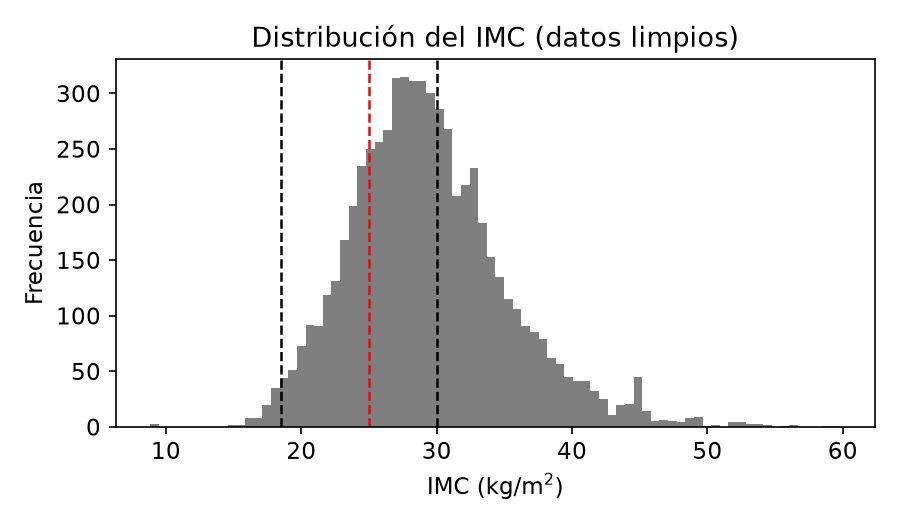
\includegraphics[width=\columnwidth]{figures/hist_imc.png}
\caption{Histograma del IMC de los datos limpios. Las líneas punteadas marcan
los cortes $18.5$, $25$ (en rojo, frontera entre $C_1$ y $C_2$) y $30$.}
\label{fig:hist}
\end{figure}

\subsection{Partición y escalamiento}
Los datos se separaron en $80\%$ para entrenamiento ($4\,997$ patrones) y
$20\%$ para prueba ($1\,249$ patrones) mediante muestreo aleatorio con
semilla fija (\texttt{random\_state=42}).

Como la altura ($\approx1.6$ m) y el peso ($\approx75$ kg) tienen escalas muy
distintas, se aplicó estandarización (\textit{standard scaling}) a cada
característica:
\begin{align}
    \label{eq:zscore}
    z_j(k)=\frac{x_j(k)-\mu_j}{\sigma_j}
\end{align}
Los parámetros obtenidos se reportan en el Cuadro~\ref{tab:escala}, junto con
los de la normalización Min--Max
\begin{align}
    \label{eq:minmax}
    \bar{x}_j(k)=\frac{x_j(k)-x_{j,\min}}{x_{j,\max}-x_{j,\min}}
\end{align}
que se usó como alternativa de comparación. Los mismos $\mu_j$ y $\sigma_j$ se
reutilizaron sin cambios para transformar el conjunto de prueba.

\begin{table}[htbp]
\caption{Parámetros de escalamiento}
\label{tab:escala}
\begin{center}
\begin{tabular}{lcccc}
\toprule
\textbf{Variable} & $\mu_j$ & $\sigma_j$ & $x_{j,\min}$ & $x_{j,\max}$ \\
\midrule
Altura (m) & $1.5948$ & $0.1078$ & $1.065$ & $2.222$ \\
Peso (kg)  & $75.279$ & $19.841$ & $32.05$ & $222.22$ \\
\bottomrule
\end{tabular}
\end{center}
\end{table}

\subsection{Diseño de la red}
La arquitectura consta de dos entradas (altura y peso estandarizados), una
sola neurona con salida lineal y un \textit{bias} $b$ representado como un
escalar independiente del vector de pesos. Los parámetros de diseño se
resumen en el Cuadro~\ref{tab:diseno}.

\begin{table}[htbp]
\caption{Parámetros de diseño de la ADALINE}
\label{tab:diseno}
\begin{center}
\begin{tabular}{ll}
\toprule
\textbf{Parámetro} & \textbf{Valor} \\
\midrule
Entradas            & $2$ (altura, peso) \\
Activación          & Identidad, $\varphi(v)=v$ \\
Inicialización      & $w_i,b\sim\mathcal{N}(0,\,0.01^2)$, semilla $1$ \\
Modalidad           & Estocástica (SGD), $M=1$ \\
Mezcla de patrones  & Sí, al inicio de cada época \\
Razón de aprendizaje& $\eta=10^{-4}$ \\
Épocas máximas      & $100$ \\
Criterio de paro    & $|E_{t}-E_{t-1}|<10^{-6}$ \\
Escalamiento        & Estandarización (z-score) \\
\bottomrule
\end{tabular}
\end{center}
\end{table}

Se eligió la modalidad estocástica: en cada época se recorren todos los
patrones en orden aleatorio y los parámetros se actualizan inmediatamente
después de cada uno con \eqref{eq:deltaW} y \eqref{eq:deltab}, por lo que hay
$N$ actualizaciones por época. Al final de cada época se registra el error
global
\begin{align}
    \label{eq:Eepoca}
    E_t=\frac{1}{2}\sum_{i=1}^{N}\left[d_i-y_i\right]^2,
\end{align}
que es proporcional al MSE ($\text{MSE}=2E_t/N$) y se usa tanto para la
curva de aprendizaje como para el criterio de paro. El entrenamiento también
se detiene si $E_t$ deja de ser finito (divergencia).

\subsection{Algoritmo}
El procedimiento implementado en Python con NumPy, sin bibliotecas de redes
neuronales, es el siguiente:
\begin{algorithmic}[1]
\STATE Inicializar $\mathbf{W}(0)$, $b(0)\sim\mathcal{N}(0,0.01^2)$
\FOR{$t=1$ \TO $100$}
    \STATE Mezclar el orden de los patrones
    \FOR{cada patrón $k$}
        \STATE $y(k)\leftarrow\mathbf{W}^\top\mathbf{X}(k)+b$
        \STATE $e(k)\leftarrow d(k)-y(k)$
        \STATE $\mathbf{W}\leftarrow\mathbf{W}+\eta\,e(k)\mathbf{X}(k)$
        \STATE $b\leftarrow b+\eta\,e(k)$
    \ENDFOR
    \STATE Calcular y guardar $E_t$ con \eqref{eq:Eepoca}
    \IF{$E_t$ no es finito \OR $|E_t-E_{t-1}|<10^{-6}$}
        \STATE Detener
    \ENDIF
\ENDFOR
\STATE Clasificar el conjunto de prueba con \eqref{eq:signo}
\end{algorithmic}

\subsection{Condición de convergencia}
Para el caso batch con paso fijo, una condición estándar es
$0<\eta<2/\lambda_{\max}(H)$ con $H=\frac{1}{N}X^\top X$ \cite{b4}. Con
entradas estandarizadas, las columnas de $X$ tienen media cero y varianza
unitaria, por lo que $H$ es la matriz de correlación entre altura y peso
(más un término unitario e independiente para el bias). Sus valores propios
son $1\pm\rho$, con $\rho$ la correlación, así que
$\lambda_{\max}\leq2$ y cualquier $\eta<1$ cumple la condición. Los valores
estudiados ($10^{-5}$ a $10^{-3}$) están muy por debajo de este límite; en
SGD, sin embargo, el ruido del gradiente estimado con un solo patrón hace que
$\eta$ también controle la amplitud de las oscilaciones alrededor del mínimo.

\section{Resultados}

\subsection{Curva de aprendizaje}
Con $\eta=10^{-4}$ el error pasó de $E_1=2\,060.6$ a $E_{100}=1\,341.0$
(Fig.~\ref{fig:mse}), equivalente a un MSE final de $0.429$. La curva decrece
rápidamente durante las primeras $\sim$10 épocas y después se estabiliza en
una meseta con variaciones muy pequeñas (desviación estándar de $0.019$ en las
últimas 10 épocas). No se observa divergencia. El criterio de paro
$|E_t-E_{t-1}|<10^{-6}$ resultó demasiado estricto para el ruido propio de SGD,
por lo que el entrenamiento terminó al alcanzar las $100$ épocas. Los
parámetros finales (en el espacio estandarizado) fueron
\begin{align*}
    \mathbf{W}=\begin{bmatrix}-0.3926 & 0.6123\end{bmatrix}^\top,\quad b=0.5610.
\end{align*}

\begin{figure}[htbp]
\centering
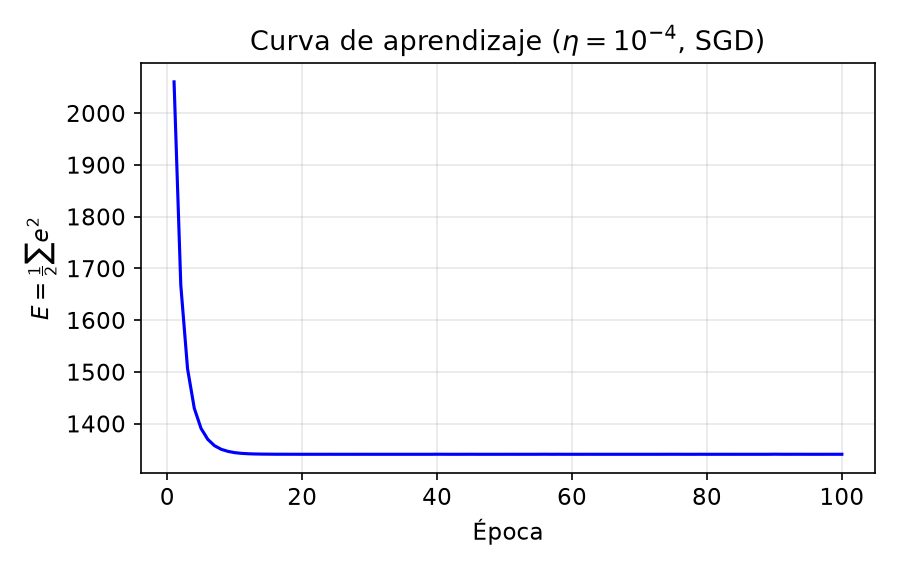
\includegraphics[width=\columnwidth]{figures/curva_mse.png}
\caption{Curva de aprendizaje del modelo final ($\eta=10^{-4}$, SGD, estandarización).}
\label{fig:mse}
\end{figure}

\subsection{Estudio de la razón de aprendizaje}
Se entrenó la red con tres valores de $\eta$, manteniendo la misma
inicialización, partición y escalamiento (Fig.~\ref{fig:eta} y
Cuadro~\ref{tab:eta}).

\begin{figure}[htbp]
\centering
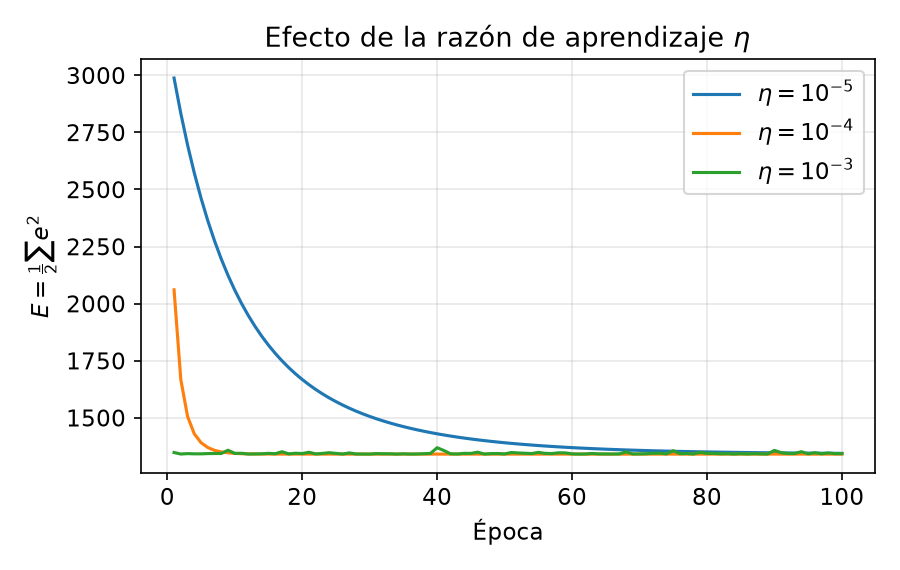
\includegraphics[width=\columnwidth]{figures/eta_comparacion.png}
\caption{Curva de error para tres valores de $\eta$.}
\label{fig:eta}
\end{figure}

\begin{table}[htbp]
\caption{Efecto de $\eta$ (100 épocas, SGD, z-score)}
\label{tab:eta}
\begin{center}
\begin{tabular}{lcccc}
\toprule
$\eta$ & $E_1$ & $E_{100}$ & $\sigma(E)$ últ. 10 & Exactitud \\
\midrule
$10^{-5}$ & $2\,988.1$ & $1\,344.1$ & $0.641$ & $87.35\%$ \\
$10^{-4}$ & $2\,060.6$ & $1\,341.0$ & $0.019$ & $88.39\%$ \\
$10^{-3}$ & $1\,347.9$ & $1\,342.9$ & $2.846$ & $88.71\%$ \\
\bottomrule
\end{tabular}
\end{center}
\end{table}

\begin{itemize}
    \item $\eta=10^{-5}$: aprendizaje estable pero lento; tras $100$ épocas la
    curva todavía no termina de descender (la variación de $0.641$ refleja el
    descenso, no oscilación).
    \item $\eta=10^{-4}$: disminución rápida y sostenida, y la meseta más estable.
    \item $\eta=10^{-3}$: alcanza el mínimo desde la primera época, pero
    presenta picos y oscilaciones alrededor de él (por ejemplo, cerca de las
    épocas 40 y 90), típico de un paso grande con gradiente estocástico.
\end{itemize}
Se seleccionó $\eta=10^{-4}$ por ofrecer el mejor compromiso entre velocidad y
estabilidad. La diferencia de exactitud con $\eta=10^{-3}$ ($0.3\%$) no
compensa su mayor oscilación.

\subsection{Comparación de escalamiento}
Con $\eta=10^{-4}$ fijo, se comparó la estandarización con la normalización
Min--Max a $[0,1]$ (Fig.~\ref{fig:escala}). Con Min--Max el error bajó solo
de $2\,323.2$ a $1\,748.3$ en $100$ épocas y la exactitud en prueba fue de
$78.38\%$, frente a $88.39\%$ con la estandarización. Min--Max produce
entradas no centradas (todas positivas) y comprimidas en un rango pequeño,
debido a valores extremos como $222.22$ kg. Esto empeora el
condicionamiento de $H$ y hace más lento el avance del gradiente. Por eso se
eligió la estandarización para el modelo final.

\begin{figure}[htbp]
\centering
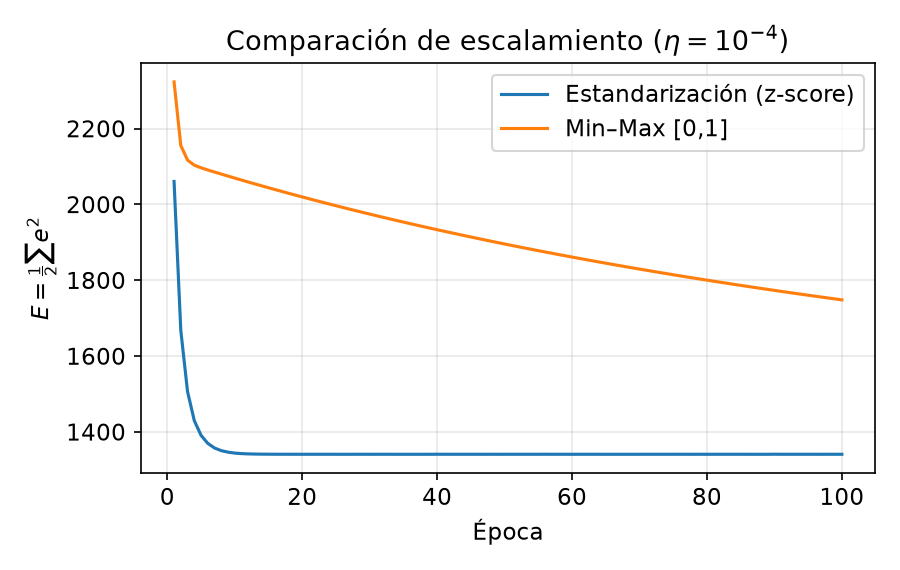
\includegraphics[width=\columnwidth]{figures/escalamiento_comparacion.png}
\caption{Curva de error con estandarización y con Min--Max ($\eta=10^{-4}$).}
\label{fig:escala}
\end{figure}

\subsection{Frontera de decisión}
En el espacio estandarizado la frontera es
$w_1z_1+w_2z_2+b=0$. Al sustituir \eqref{eq:zscore} y despejar el peso se
obtiene la recta en unidades originales
\begin{align}
    \label{eq:frontera}
    m=\mu_2-\frac{\sigma_2}{w_2}\left(w_1\frac{h-\mu_1}{\sigma_1}+b\right)
    \approx 118.0\,h-131.1
\end{align}
con $h$ en metros y $m$ en kilogramos. La Fig.~\ref{fig:frontera} la compara
con la frontera teórica $m=25h^2$. Ambas se cruzan en $h\approx1.79$ m. Para
alturas menores, que concentran a la mayoría de la población, la recta de
ADALINE queda \emph{por debajo} de la parábola, así que personas con IMC
ligeramente menor que $25$ se clasifican como $C_2$. La pendiente de la recta
($118$ kg/m) es mayor que la de la tangente a la parábola en la altura media
($50h\approx80$ kg/m en $h=1.6$ m).

\begin{figure}[htbp]
\centering
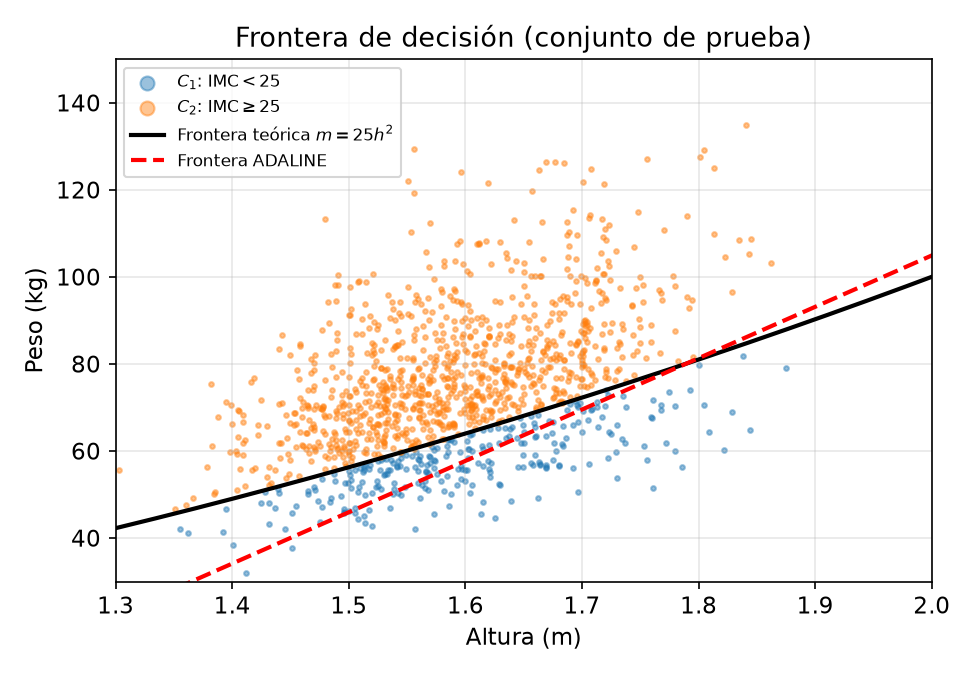
\includegraphics[width=\columnwidth]{figures/frontera.png}
\caption{Patrones de prueba, frontera aprendida por ADALINE (rojo, punteada)
y frontera teórica IMC $=25$ (negro).}
\label{fig:frontera}
\end{figure}

\subsection{Generalización}
En los $1\,249$ patrones de prueba la exactitud fue
\begin{align*}
    \text{Accuracy}=\frac{125+979}{1\,249}=88.39\%.
\end{align*}
La matriz de confusión (Fig.~\ref{fig:cm}) muestra que \emph{todos} los
errores son del tipo $C_1$ clasificados como $C_2$ ($145$), mientras que
ningún patrón de $C_2$ se clasificó como $C_1$. La sensibilidad de $C_2$ es
de $100\%$ y la de $C_1$ es de solo $46.3\%$ ($125/270$).

\begin{figure}[htbp]
\centering
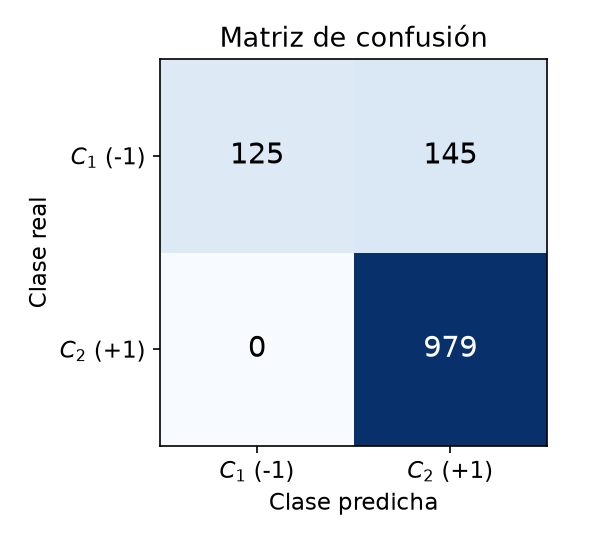
\includegraphics[width=0.8\columnwidth]{figures/matriz_confusion.png}
\caption{Matriz de confusión en el conjunto de prueba.}
\label{fig:cm}
\end{figure}

Para verificar que los errores se concentran cerca de la frontera, se contó
cuántos patrones mal clasificados tienen un IMC cercano a $25$
(Cuadro~\ref{tab:errores}). El $87.6\%$ de los errores ocurre en
$|\text{IMC}-25|<3$.

\begin{table}[htbp]
\caption{Errores de prueba cerca de IMC $=25$}
\label{tab:errores}
\begin{center}
\begin{tabular}{lccc}
\toprule
\textbf{Banda} & \textbf{Patrones} & \textbf{Errores} & \textbf{\% del total de errores} \\
\midrule
$|\text{IMC}-25|<1$ & $138$ & $60$  & $41.4\%$ \\
$|\text{IMC}-25|<2$ & $294$ & $107$ & $73.8\%$ \\
$|\text{IMC}-25|<3$ & $423$ & $127$ & $87.6\%$ \\
\bottomrule
\end{tabular}
\end{center}
\end{table}

\section{Discusión}

\textbf{Error con la salida lineal.} ADALINE calcula el error con $y(k)$ y no
con la salida de la función signo porque esta última no es diferenciable y su
derivada es cero casi en todas partes. Con la salida lineal, $E$ es una
función cuadrática y suave de $\mathbf{W}$ y $b$, cuyo gradiente da la regla
delta. Además, el error lineal indica \emph{qué tan lejos} está el patrón de la
frontera, no solo si está bien o mal clasificado.

\textbf{Efecto de $\eta$ y del escalamiento.} Un $\eta$ pequeño hace
la convergencia lenta y uno grande la vuelve ruidosa. La estandarización
centró los datos y equilibró las escalas, lo que permitió usar un mismo $\eta$
para ambos pesos. Min--Max, con entradas no centradas, convergió mucho más
lento con el mismo $\eta$.

\textbf{Frontera aprendida vs.\ teórica.} No debe esperarse una coincidencia
exacta. La frontera real $m=25h^2$ es no lineal y ADALINE solo puede
representar rectas. Además, ADALINE no minimiza el número de errores de
clasificación, sino el error cuadrático respecto a las etiquetas $\pm1$. Ese
error lo dominan los patrones lejanos a la frontera, sobre todo los de
obesidad, que son abundantes. Como $78\%$ de los datos pertenece a $C_2$,
el término de bias se desplaza hacia $+1$ y la recta baja respecto a la
parábola. Esto explica que todos los errores sean falsos $C_2$ y que la mayoría se
concentre en IMC entre $22$ y $25$.

\textbf{Limitaciones.}
\begin{itemize}
    \item El modelo lineal no puede representar la curvatura de la frontera
    real ni separar más de dos regiones.
    \item El desbalance de clases sesga la frontera hacia la clase
    mayoritaria; una ponderación por clase o un muestreo balanceado podría
    mejorar la sensibilidad de $C_1$.
    \item En la implementación, $\mu_j$ y $\sigma_j$ se calcularon con toda
    la base, y el entrenamiento se realizó sobre los $6\,246$ patrones
    estandarizados, no solo sobre los $4\,997$ de entrenamiento. Por lo tanto, el
    conjunto de prueba no estuvo completamente aislado y la exactitud
    reportada es ligeramente optimista. Con solo tres parámetros libres el
    efecto esperado es pequeño, pero debe corregirse ajustando el escalamiento
    y el entrenamiento solo con la partición de entrenamiento.
    \item El filtro de rango de peso y estatura no eliminó $44$ registros con
    los códigos de no respuesta $222.22$ kg o $222.2$ cm, que actúan como
    valores atípicos.
    \item El criterio de paro de $10^{-6}$ sobre $E_t$ no es alcanzable con SGD;
    un umbral relativo o una paciencia de varias épocas sería más adecuado.
\end{itemize}

\textbf{SGD, mini-batch y batch.} En SGD hay $N=6\,246$ actualizaciones por
época, en mini-batch $\approx N/M$ y en batch solo una. SGD avanza más por
época, como se observa en la caída de la curva en menos de 10 épocas, pero su
curva es ruidosa. Batch daría una curva monótona y suave, pero necesitaría más
épocas para el mismo $\eta$. Mini-batch ofrece un punto intermedio.

\section{Conclusiones}
Se implementó desde cero una ADALINE entrenada con la regla delta en modalidad
estocástica, que alcanzó una exactitud de $88.39\%$ al clasificar el estado de
peso de adultos de la ENSANUT 2022 usando solo altura y peso. La curva de
aprendizaje mostró una convergencia rápida y estable con $\eta=10^{-4}$, y el
estudio de $\eta$ y del escalamiento confirmó que la estandarización y una
razón de aprendizaje moderada son determinantes para el buen
condicionamiento del problema.

El modelo aprendió una aproximación lineal razonable de la frontera $m=25h^2$
en el rango de alturas más frecuente, pero no puede representar su curvatura.
Sus errores se concentran cerca de IMC $=25$ y todos favorecen a la clase
mayoritaria. Una red multicapa con activaciones no lineales podría
aproximar la frontera curva y, con varias salidas, separar las cuatro
categorías originales del IMC, que es el siguiente paso natural de este
trabajo.

\begin{thebibliography}{00}

\bibitem{b1} S. Haykin, \textit{Neural Networks and Learning Machines}, 3rd ed. Upper Saddle River, NJ, USA: Pearson/Prentice Hall, 2009.

\bibitem{b2} B. Mehlig, \textit{Machine Learning with Neural Networks}, 2021. arXiv:1901.05639v4 [cs.LG].

\bibitem{b3} C. C. Aggarwal, \textit{Neural Networks and Deep Learning: A Textbook}. Cham, Switzerland: Springer, 2018.

\bibitem{b4} I. Goodfellow, Y. Bengio, and A. Courville, \textit{Deep Learning}. Cambridge, MA, USA: MIT Press, 2016.

\bibitem{b5} P. Isasi Viñuela and I. M. Galván León, \textit{Redes de Neuronas Artificiales: Un Enfoque Práctico}. Madrid, España: Pearson Educación, 2004.

\bibitem{b6} Instituto Nacional de Salud Pública, ``Encuesta Nacional de Salud y Nutrición Continua 2022 (ENSANUT 2022): base de datos de antropometría,'' Cuernavaca, México: INSP, 2023. [En línea]. Disponible: https://ensanut.insp.mx

\end{thebibliography}

\end{document}
